%% abtex2-modelo-trabalho-academico.tex, v-1.7.1 laurocesar
%% Copyright 2012-2013 by abnTeX2 group at http://abntex2.googlecode.com/ 
%%
%% This work may be distributed and/or modified under the
%% conditions of the LaTeX Project Public License, either version 1.3
%% of this license or (at your option) any later version.
%% The latest version of this license is in
%%   http://www.latex-project.org/lppl.txt
%% and version 1.3 or later is part of all distributions of LaTeX
%% version 2005/12/01 or later.
%%
%% This work has the LPPL maintenance status `maintained'.
%% 
%% The Current Maintainer of this work is the abnTeX2 team, led
%% by Lauro César Araujo. Further information are available on 
%% http://abntex2.googlecode.com/
%%
%% This work consists of the files abntex2-modelo-trabalho-academico.tex,
%% abntex2-modelo-include-comandos and abntex2-modelo-references.bib
%%

% ------------------------------------------------------------------------
% ------------------------------------------------------------------------
% abnTeX2: Modelo de Trabalho Academico (tese de doutorado, dissertacao de
% mestrado e trabalhos monograficos em geral) em conformidade com 
% ABNT NBR 14724:2011: Informacao e documentacao - Trabalhos academicos -
% Apresentacao
% ------------------------------------------------------------------------
% ------------------------------------------------------------------------

\documentclass[
	% -- opções da classe memoir --
	12pt,				% tamanho da fonte
	openright,			% capítulos começam em pág ímpar (insere página vazia caso preciso)
	oneside,			% para impressão em verso e anverso. Oposto a oneside
	a4paper,			% tamanho do papel. 
	% -- opções da classe abntex2 --
	%chapter=TITLE,		% títulos de capítulos convertidos em letras maiúsculas
	%section=TITLE,		% títulos de seções convertidos em letras maiúsculas
	%subsection=TITLE,	% títulos de subseções convertidos em letras maiúsculas
	%subsubsection=TITLE,% títulos de subsubseções convertidos em letras maiúsculas
	% -- opções do pacote babel --
	english,			% idioma adicional para hifenização
	french,				% idioma adicional para hifenização
	spanish,			% idioma adicional para hifenização
	brazil,				% o último idioma é o principal do documento
	]{abntex2}


% ---
% PACOTES
% ---

% ---
% Pacotes fundamentais 
% ---
\usepackage{cmap}				% Mapear caracteres especiais no PDF
\usepackage{lmodern}			% Usa a fonte Latin Modern			
\usepackage[T1]{fontenc}		% Selecao de codigos de fonte.
\usepackage[utf8]{inputenc}		% Codificacao do documento (conversão automática dos acentos)
\usepackage{lastpage}			% Usado pela Ficha catalográfica
\usepackage{indentfirst}		% Indenta o primeiro parágrafo de cada seção.
\usepackage{color}				% Controle das cores
\usepackage{graphicx}			% Inclusão de gráficos
% ---
		
% ---
% Pacotes adicionais, usados apenas no âmbito do Modelo Canônico do abnteX2
% ---
\usepackage{lipsum}				% para geração de dummy text
% ---

% ---
% Pacotes de citações
% ---
\usepackage[brazilian,hyperpageref]{backref}	 % Paginas com as citações na bibl
\usepackage[alf]{abntex2cite}	% Citações padrão ABNT

% --- 
% CONFIGURAÇÕES DE PACOTES
% --- 

% ---
% Configurações do pacote backref
% Usado sem a opção hyperpageref de backref
\renewcommand{\backrefpagesname}{Citado na(s) página(s):~}
% Texto padrão antes do número das páginas
\renewcommand{\backref}{}
% Define os textos da citação
\renewcommand*{\backrefalt}[4]{
	\ifcase #1 %
		Nenhuma citação no texto.%
	\or
		Citado na página #2.%
	\else
		Citado #1 vezes nas páginas #2.%
	\fi}%
% ---


% ---
% Informações de dados para CAPA e FOLHA DE ROSTO
% ---
\titulo{Apostila de Banco de Dados}
\autor{Isabelle Neves Porto}
\local{Brasil}
\data{2021}
% ---


% ---
% Configurações de aparência do PDF final

% alterando o aspecto da cor azul
\definecolor{blue}{RGB}{41,5,195}

% informações do PDF
\makeatletter
\hypersetup{
     	%pagebackref=true,
		pdftitle={\@title}, 
		pdfauthor={\@author},
    	pdfsubject={\imprimirpreambulo},
	    pdfcreator={LaTeX with abnTeX2},
		pdfkeywords={abnt}{latex}{abntex}{abntex2}{trabalho acadêmico}, 
		colorlinks=true,       		% false: boxed links; true: colored links
    	linkcolor=blue,          	% color of internal links
    	citecolor=blue,        		% color of links to bibliography
    	filecolor=magenta,      		% color of file links
		urlcolor=blue,
		bookmarksdepth=4
}
\makeatother
% --- 

% --- 
% Espaçamentos entre linhas e parágrafos 
% --- 

% O tamanho do parágrafo é dado por:
\setlength{\parindent}{1.3cm}

% Controle do espaçamento entre um parágrafo e outro:
\setlength{\parskip}{0.2cm}  % tente também \onelineskip

% ---
% compila o indice
% ---
\makeindex
% ---

% ----
% Início do documento
% ----
\begin{document}

% Retira espaço extra obsoleto entre as frases.
\frenchspacing 

% ----------------------------------------------------------
% ELEMENTOS PRÉ-TEXTUAIS
% ----------------------------------------------------------
% \pretextual

% ---
% Capa
% ---
\imprimircapa
% ---

% ---
% inserir lista de ilustrações
% ---
\pdfbookmark[0]{\listfigurename}{lof}
\listoffigures*
\cleardoublepage
% ---

% ---
% inserir lista de tabelas
% ---
\pdfbookmark[0]{\listtablename}{lot}
\listoftables*
\cleardoublepage
% ---

% ---
% inserir lista de abreviaturas e siglas
% ---
\begin{siglas}
  \item[SGBD] Sistema Gerenciador de Banco de Dados
  \item[DBA] Database Administrator
  \item[SQL] Standard Query Language
\end{siglas}
% ---

% ---
% inserir lista de símbolos
% ---
%%\begin{simbolos}
%%  \item[$ \Gamma $] Letra grega Gama
%%  \item[$ \Lambda $] Lambda
%%  \item[$ \zeta $] Letra grega minúscula zeta
%%  \item[$ \in $] Pertence
%%\end{simbolos}
% ---

% ---
% inserir o sumario
% ---
\pdfbookmark[0]{\contentsname}{toc}
\tableofcontents*
\cleardoublepage
% ---



% ----------------------------------------------------------
% ELEMENTOS TEXTUAIS
% ----------------------------------------------------------
\textual

% ----------------------------------------------------------
% Introdução
% ----------------------------------------------------------
\chapter*[Introdução]{Introdução}
\addcontentsline{toc}{chapter}{Introdução}

Um banco de dados é uma coleção de dados. Um dado pode ser um fato sobre qualquer objeto em consideração (nome, idade e altura são dados relacionados a você), sendo um fato que deve ser armazenado/persistido e que tem um significado implícito.

Nós vamos estudar dois tipos de banco de dados: os relacionais e os não relacionais.

Os bancos relacionais são compostos por tabelas que relacionam os dados entre eles, sendo um exemplo de banco de dados relacional o PostgresSQL, o MySQL e o SQL Server.

Os bancos não relacionais utilizam uma estrutura de dados diferente do banco relacional, não dispondo de tabelas e sim coleções de dados no lugar. Nós veremos o que isso significa mais para frente. Exemplos de bancos não relacionais são o MongoDB, DynamoDB e Cassandra.

Nós chamamos de DBA (\textit{Database Administrator}, administrador de banco de dados) o profissional que dentro de uma equipe de tecnologia é responsável por criar, manter e otimizar banco de dados.

\part{Bancos Relacionais}

\chapter{Introdução}

Os dados armazenados nos bancos relacionais são organizados por tabelas. Essas tabelas possuem linhas e colunas, com cada célula representando o valor de um dado. Uma linha pode ser chamada de registro e contém uma instância exclusiva de dados \cite{sqlenosql}. Um exemplo de representação de uma tabela pode ser visto na figura \ref{fig:tabelarelacional}.

\begin{figure}[h!]
  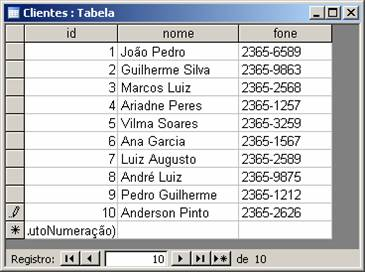
\includegraphics[scale=1]{Imagens/tabela.jpg}
  \caption{Uma tabela de banco de dados relacional}
  \label{fig:tabelarelacional}
\end{figure}

Existem softwares que criam isso no mundo computacional. Da mesma forma que existe o Excel, que salva dados em planilhas, existe os SGBD (Sistema Gerenciador de Banco de Dados), que manipulam banco de dados relacionais.

Um SGBD é um software que permite que seu usuário crie e mantenha um banco de dados. É um sistema que permite duas ações principais: 

 \begin{itemize}
   \item \textbf{Definir um banco de dados:} criar as estruturas para armazenamento dos dados e especificar as restrições que devem ser impostas aos dados;
   \item \textbf{Manipular os dados dos banco de dados:} consultar, inserir, alterar e excluir dados do banco de dados.
 \end{itemize}
 
Nessa apostila nós iremos nos basear no funcionamento do SGBD PostgreSQL. Para baixá-lo, visite \href{https://www.enterprisedb.com/downloads/postgres-postgresql-downloads}{esse site}.

\chapter{SQL}

SQL significa Standard Query Language, e é uma linguagem padrão para trabalhar com bancos de dados relacionais. Cada SGBD tem sua implementação do SQL, mas de forma geral, os comandos são muito parecidos entre todos os bancos relacionais.

Nós chamamos de \textit{query} uma consulta feita ao banco de dados, através da linguagem SQL. Exemplos de \textit{queries} são listagem de dados, atualização de dados e deleção de dados.

\section{\textit{Queries} de criação de tabelas}

Para passar a salvar os dados em uma tabela, nós precisamos primeiro definir essa tabela para o SGBD. Isso é feito através do comando CREATE TABLE, como exemplificado abaixo: 
\begin{verbatim}
CREATE TABLE pessoa (
    id INTEGER PRIMARY KEY,
    nome VARCHAR(50)
);

CREATE TABLE disciplina (
    nome VARCHAR(50),
    carga_horaria INTEGER
);
\end{verbatim}

A estrutura do comando é a seguinte: após o ``CREATE TABLE'', você coloca o nome que você quer dar à sua tabela. Dentro dos parenteses você vai declarar as colunas dessa sua tabela, escrevendo o nome da coluna seguido pelo tipo de dado que ela vai armazenar. Os tipos de dados disponíveis mais comuns são:

\begin{table}[htb]
\center
\footnotesize
\begin{tabular}{|p{3cm}|p{9cm}|}
  \hline
   \textbf{Tipo de dado} & \textbf{Significado} \\
    \hline
    INTEGER & Armazena números inteiros \\
    \hline
    NUMERIC & Armazena números fracionários \\
    \hline
    VARCHAR(N) & Armazena caracteres com o tamanho máximo definido (N) \\
    \hline
    TEXT & Armazena caracteres sem limite de tamanho \\
    \hline
    DATE & Armazena uma data \\
    \hline
    TIMESTAMP & Armazena uma data com horário \\
    \hline
    BOOLEAN & Armazena um valor booleano (verdadeiro ou falso) \\
   \hline
\end{tabular}
\caption{Tabela com lista dos tipos de dados mais comuns no PostgreSQL}
\label{tiposdedados}
\end{table}

Não pode existir duas tabelas com o mesmo nome, portanto caso você tente executar o mesmo comando de criação de tabela duas vezes, ele vai falhar na segunda vez. Também não é possível ter duas colunas na mesma tabela com o mesmo nome. 

Na tabela pessoa, um dos campos está marcado como PRIMARY KEY. Isso significa que esse campo vai ser a chave primária dessa tabela. A chave primária de uma tabela é a coluna que possui o valor que vai identificar a instância de dados dentro da tabela, possuindo um valor único para cada linha. Funciona da mesma forma que o CPF para as pessoas no Brasil: é um valor único que identifica quem é essa pessoa. Não é possível inserir no banco de dados duas linhas em uma tabela com o mesmo valor para a chave primária: fazer isso seria como repetir o CPF de alguém para outra pessoa.

\section{\textit{Queries} de inserção de dados}

Para inserir dados em uma tabela, é usado o comando ``INSERT INTO''. Exemplo usando as tabelas citadas anteriormente: 
\begin{verbatim}
INSERT INTO pessoa VALUES (1, `Isabelle');
INSERT INTO disciplina VALUES (`Back-end', 150);
\end{verbatim}

Dentro de ``VALUES'' é colocado o valor que corresponde a cada coluna. Nesse caso, é necessário passar os valores na ordem que as colunas foram criadas. Caso você não queira usar a mesma ordem ou não queira preencher alguma coluna específica, pode executar o comando especificando as colunas dessa forma:
\begin{verbatim}
INSERT INTO pessoa(id) VALUES (2);
INSERT INTO disciplina(carga_horaria, nome) VALUES (100, `Banco de dados');
\end{verbatim}

\section{\textit{Queries} de seleção de dados}

Para selecionar os dados de uma tabela, nós usamos o comando SELECT, seguindo a sintaxe abaixo:
\begin{verbatim}
SELECT * FROM tabela;
\end{verbatim}

Esse comando irá trazer todos os dados da tabela chamada ``tabela''. O asterisco (*) apresentado na \textit{query} representa a seleção de todas as colunas da tabela. Para selecionar colunas específicas, nós podemos fazer o seguinte:
\begin{verbatim}
SELECT id, nome FROM pessoa;
SELECT carga_horaria FROM disciplina;
\end{verbatim}

Dessa forma, nós ainda estamos trazendo todos as linhas da tabela, porém agora estamos trazendo colunas específicas. Para especificar linhas da tabelas, nós podemos estipular condições. Essas condições são implementadas no SQL através da cláusula WHERE. Um exemplo seria:

\begin{verbatim}
SELECT * FROM pessoa WHERE nome = `Isabelle';
SELECT id FROM disciplina WHERE carga_horaria > 100;
\end{verbatim}

No primeiro exemplo nós estamos listando todos os dados das pessoas com o nome igual a Isabelle. No segundo exemplo nós estamos listando o id das disciplinas com carga horária maior que 100. Os operadores que nós podemos usar para criar condições são:

\begin{itemize}
   \item \textbf{=} restringe para linhas com o valor igual ao especificado;
   \begin{verbatim}
   SELECT * FROM pessoa WHERE nome = `Isabelle';
   \end{verbatim}
   
   \item \textbf{\textgreater{} e \textless{}} usado para colunas numéricas, restringe a valores maiores/menores que o especificado;
   \begin{verbatim}
   SELECT * FROM disciplina WHERE carga_horaria > 100;
   \end{verbatim}
   
   \item \textbf{\textgreater{}= e \textless{}=} usado para colunas numéricas, restringe a valores maiores ou iguais ao especificado;
   \begin{verbatim}
   SELECT * FROM disciplina WHERE carga_horaria <= 100;
   \end{verbatim}
   
   \item \textbf{IN} usado para restringir a um conjunto de valores;
   \begin{verbatim}
   SELECT * FROM disciplina WHERE nome IN (`Banco de dados', `Back-end');
   \end{verbatim}
\end{itemize}
 
Além de ter condições simples para a consulta, nós podemos também mesclar essas condições, através dos operadores AND e OR.
\begin{verbatim}
SELECT * FROM pessoa WHERE idade > 18 AND nome = `Isabelle';
SELECT * FROM disciplina WHERE nome = `Back-end' OR carga_horaria = 100;
\end{verbatim}

Na primeira consulta nós estamos buscando por todas as pessoas com nome igual a ``Isabelle'' e com idade acima de 18. Na segunda consulta nós estamos buscando por todas as disciplinas cujo nome é igual a ``Back-end'' ou a carga horária é maior que 100, retornando todas as que baterem com pelo menos uma das condições especificadas.

Além dos operadores já apresentados, nós temos também as chamadas ``funções de agregação''. Funções de agregação são o que permite a execução de uma operação aritmética nos valores de uma coluna considerando todos os registros de uma tabela \cite{agregacao}. As funções de agregação mais utilizadas são as seguintes:

\begin{itemize}
   \item \textbf{COUNT: } conta quantos registros essa consulta retornaria. No exemplo, o retorno vai ser o número de pessoas com o nome ``Isabelle'':
   \begin{verbatim}
   SELECT COUNT(*) FROM pessoa WHERE nome = `Isabelle';
   \end{verbatim}
   
   \item \textbf{MAX e MIN: } usado para colunas numéricas, retorna qual o valor máximo/mínimo que a coluna atingiu dentre todos os registros que correspondem com a condição especificada. No exemplo, irá ser retornado qual é o valor máximo de carga horária entre todas as disciplinas:
   \begin{verbatim}
   SELECT MAX(carga_horaria) FROM disciplina;
   \end{verbatim}
   
   \item \textbf{AVG: } usado para colunas numéricas, ele serve para calcular a média do valor de uma coluna dentre todas as linhas que correspondem com a condição especificada. No exemplo, será calculado a média de idade das pessoas com o nome ``Isabelle'':
   \begin{verbatim}
   SELECT AVG(carga_horaria) FROM disciplina;
   \end{verbatim}
   
   \item \textbf{SUM: } usado para colunas numéricas, retorna a soma dos valores de determinada coluna de todos os registros que correspondem com a condição especificada. O exemplo retorna a soma da carga horária das matérias de nome ``Banco de dados'' e ``Back-end'':
   \begin{verbatim}
   SELECT SUM(carga_horaria) FROM disciplina WHERE nome IN (`Banco de 
   dados', `Back-end');
   \end{verbatim}
\end{itemize}

% ---
% Finaliza a parte no bookmark do PDF, para que se inicie o bookmark na raiz
% ---
\bookmarksetup{startatroot}% 
% ---

% ----------------------------------------------------------
% ELEMENTOS PÓS-TEXTUAIS
% ----------------------------------------------------------
\postextual


% ----------------------------------------------------------
% Referências bibliográficas
% ----------------------------------------------------------
\bibliography{abntex2-modelo-references}

% ----------------------------------------------------------
% Glossário
% ----------------------------------------------------------
%
% Consulte o manual da classe abntex2 para orientações sobre o glossário.
%
%\glossary

% ----------------------------------------------------------
% Apêndices
% ----------------------------------------------------------

% ---
% Inicia os apêndices
% ---
%%\begin{apendicesenv}

% Imprime uma página indicando o início dos apêndices
%%\partapendices

% ----------------------------------------------------------
%%\chapter{Quisque libero justo}
% ----------------------------------------------------------

%%\end{apendicesenv}
% ---


% ----------------------------------------------------------
% Anexos
% ----------------------------------------------------------

% ---
% Inicia os anexos
% ---
%%\begin{anexosenv}

% Imprime uma página indicando o início dos anexos
%%\partanexos

% ---
%%\chapter{Morbi ultrices rutrum lorem.}
% ---

%%\end{anexosenv}

%---------------------------------------------------------------------
% INDICE REMISSIVO
%---------------------------------------------------------------------

\printindex

\end{document}
